\chapter{Firmware}

\subsection{Code flow}
In arduino's "version" of C there are two main structural components to the code. The void setup and the void loop. In the setup the necessary initialisations are done such as the setup of the serial communication and required output pins. The loop runs over and over again as the name implies. The implemented code inside this loop includes Reading in ADC analogue values and then converting \& calibrating those values to their practical values. After this step the necessary steps are taken to read in strings from the serial input. When reading strings from serial each character is received individually. A while loop is used to append each character to a single string. Depending on the received string the over charge control will be changed. All calibrated values and the status of the charging is then printed to serial, then there is a second delay after which the loop is repeated again.

\begin{figure}[!htb]
	\centering
	\includegraphics[width=0.5\linewidth]{Figures/A8/flowfirmware.png}
	\caption{Firmware flow diagram}
	\label{fig:flow}
\end{figure}

\subsection{Calibration of ADC}
Using $V_{in}=(\frac{5V\times ADC_{val} }{1023})$ the ADC values are converted to the input voltages at the ADC. Then this value is used uniquely for each adc measurement to get the representative value. All the methods of calibration are linearly done. The measured \textbf{calibration points} for all adc calibrations can all be see in the respective figures.






\begin{wrapfigure}{l}{0.38\textwidth}
	\begin{center}
		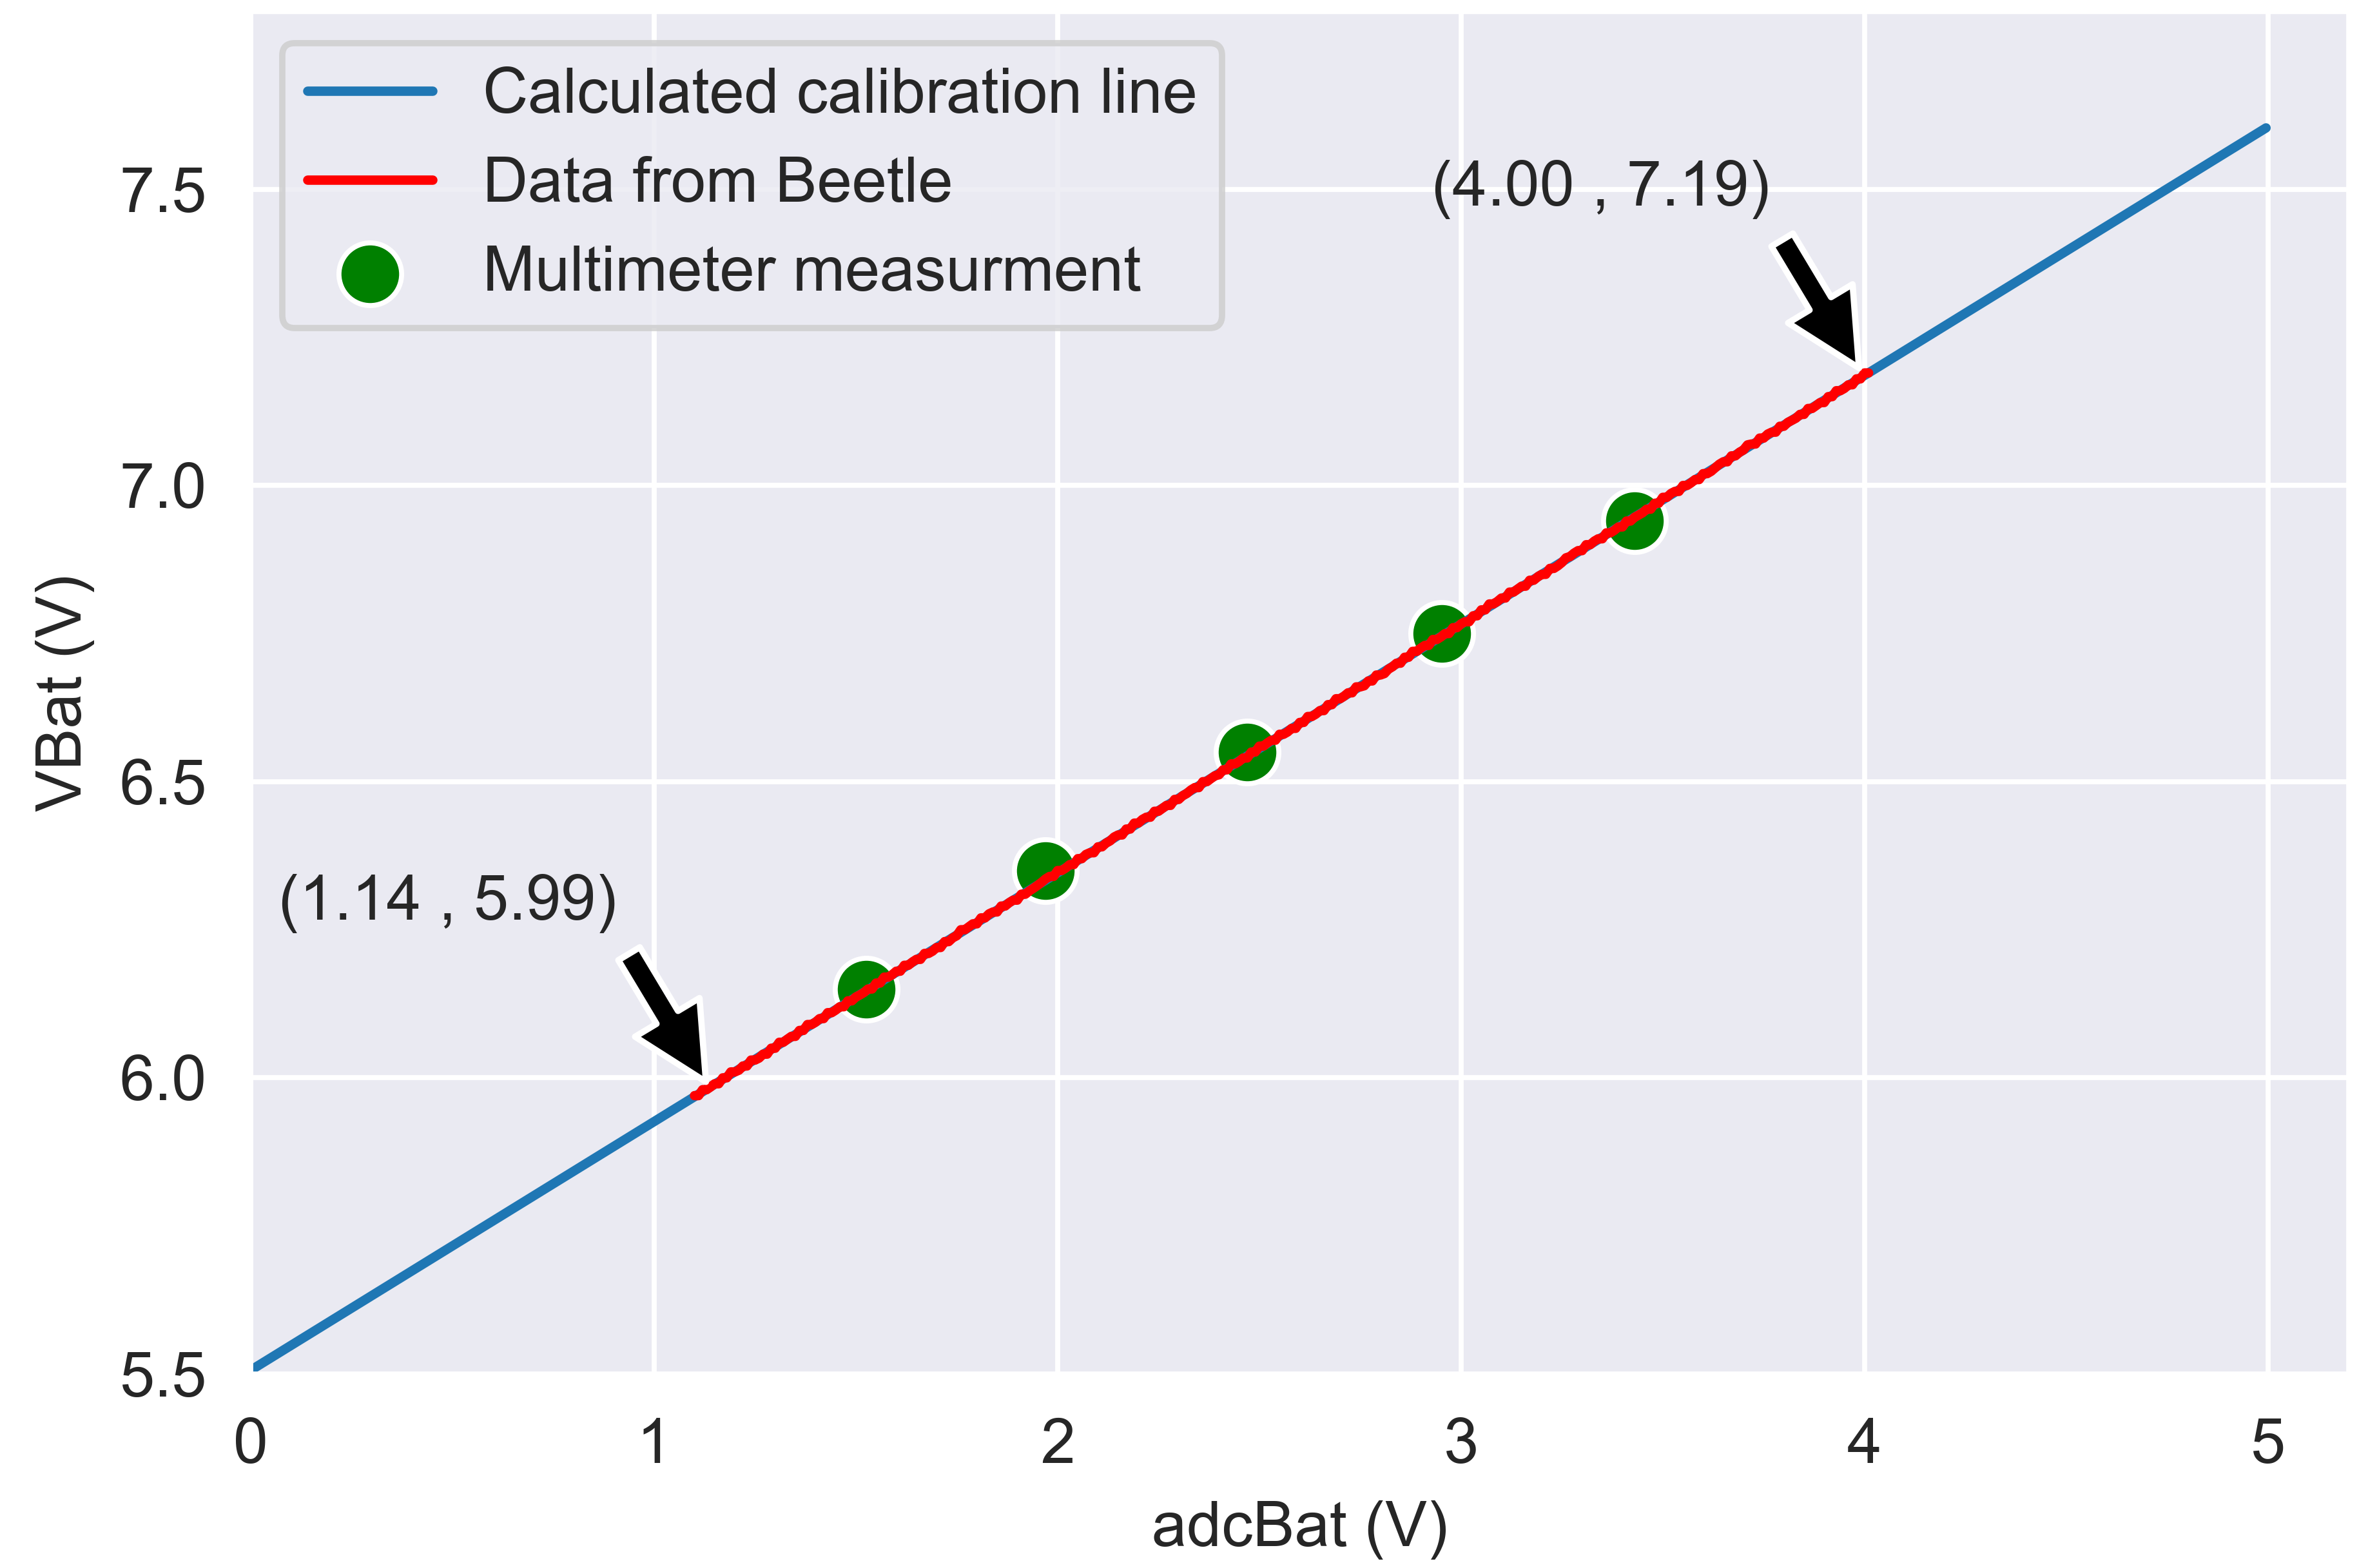
\includegraphics[width=0.38\textwidth]{./Figures/A8/batteryA8.png}
	\end{center}
	\caption{Battery ADC calibration}
	\label{fig:A8bat}
\end{wrapfigure}
Using the below equation the \textbf{battery ADC} is calibrated to be the same as the measured values. The equation is the line equation $y-y_1=(\frac{y_1-y_0}{x_1-x_0})\times x$. \newline
$V_{Bat}=(V_{adcBat}-V_{adcMax})\times \frac{(V_{batMax}-V_{batMin})}{(V_{adcHMeas}-V_{adcLMeas})}+V_{batMax}$. $V_{adcHMeas}$ and $V_{adcLMeas}$ are voltages measured at the battery adc input when the battery voltage is at its min an max value. $V_{batADC}$ is the calculated input voltage that the arduino beetle is receiving. In figure \ref{fig:A8bat} the data from the beetle is shown in comparison to multimeter measurements and it can be said that the calibration equation worked.



\begin{wrapfigure}{l}{0.38\textwidth}
	\begin{center}
		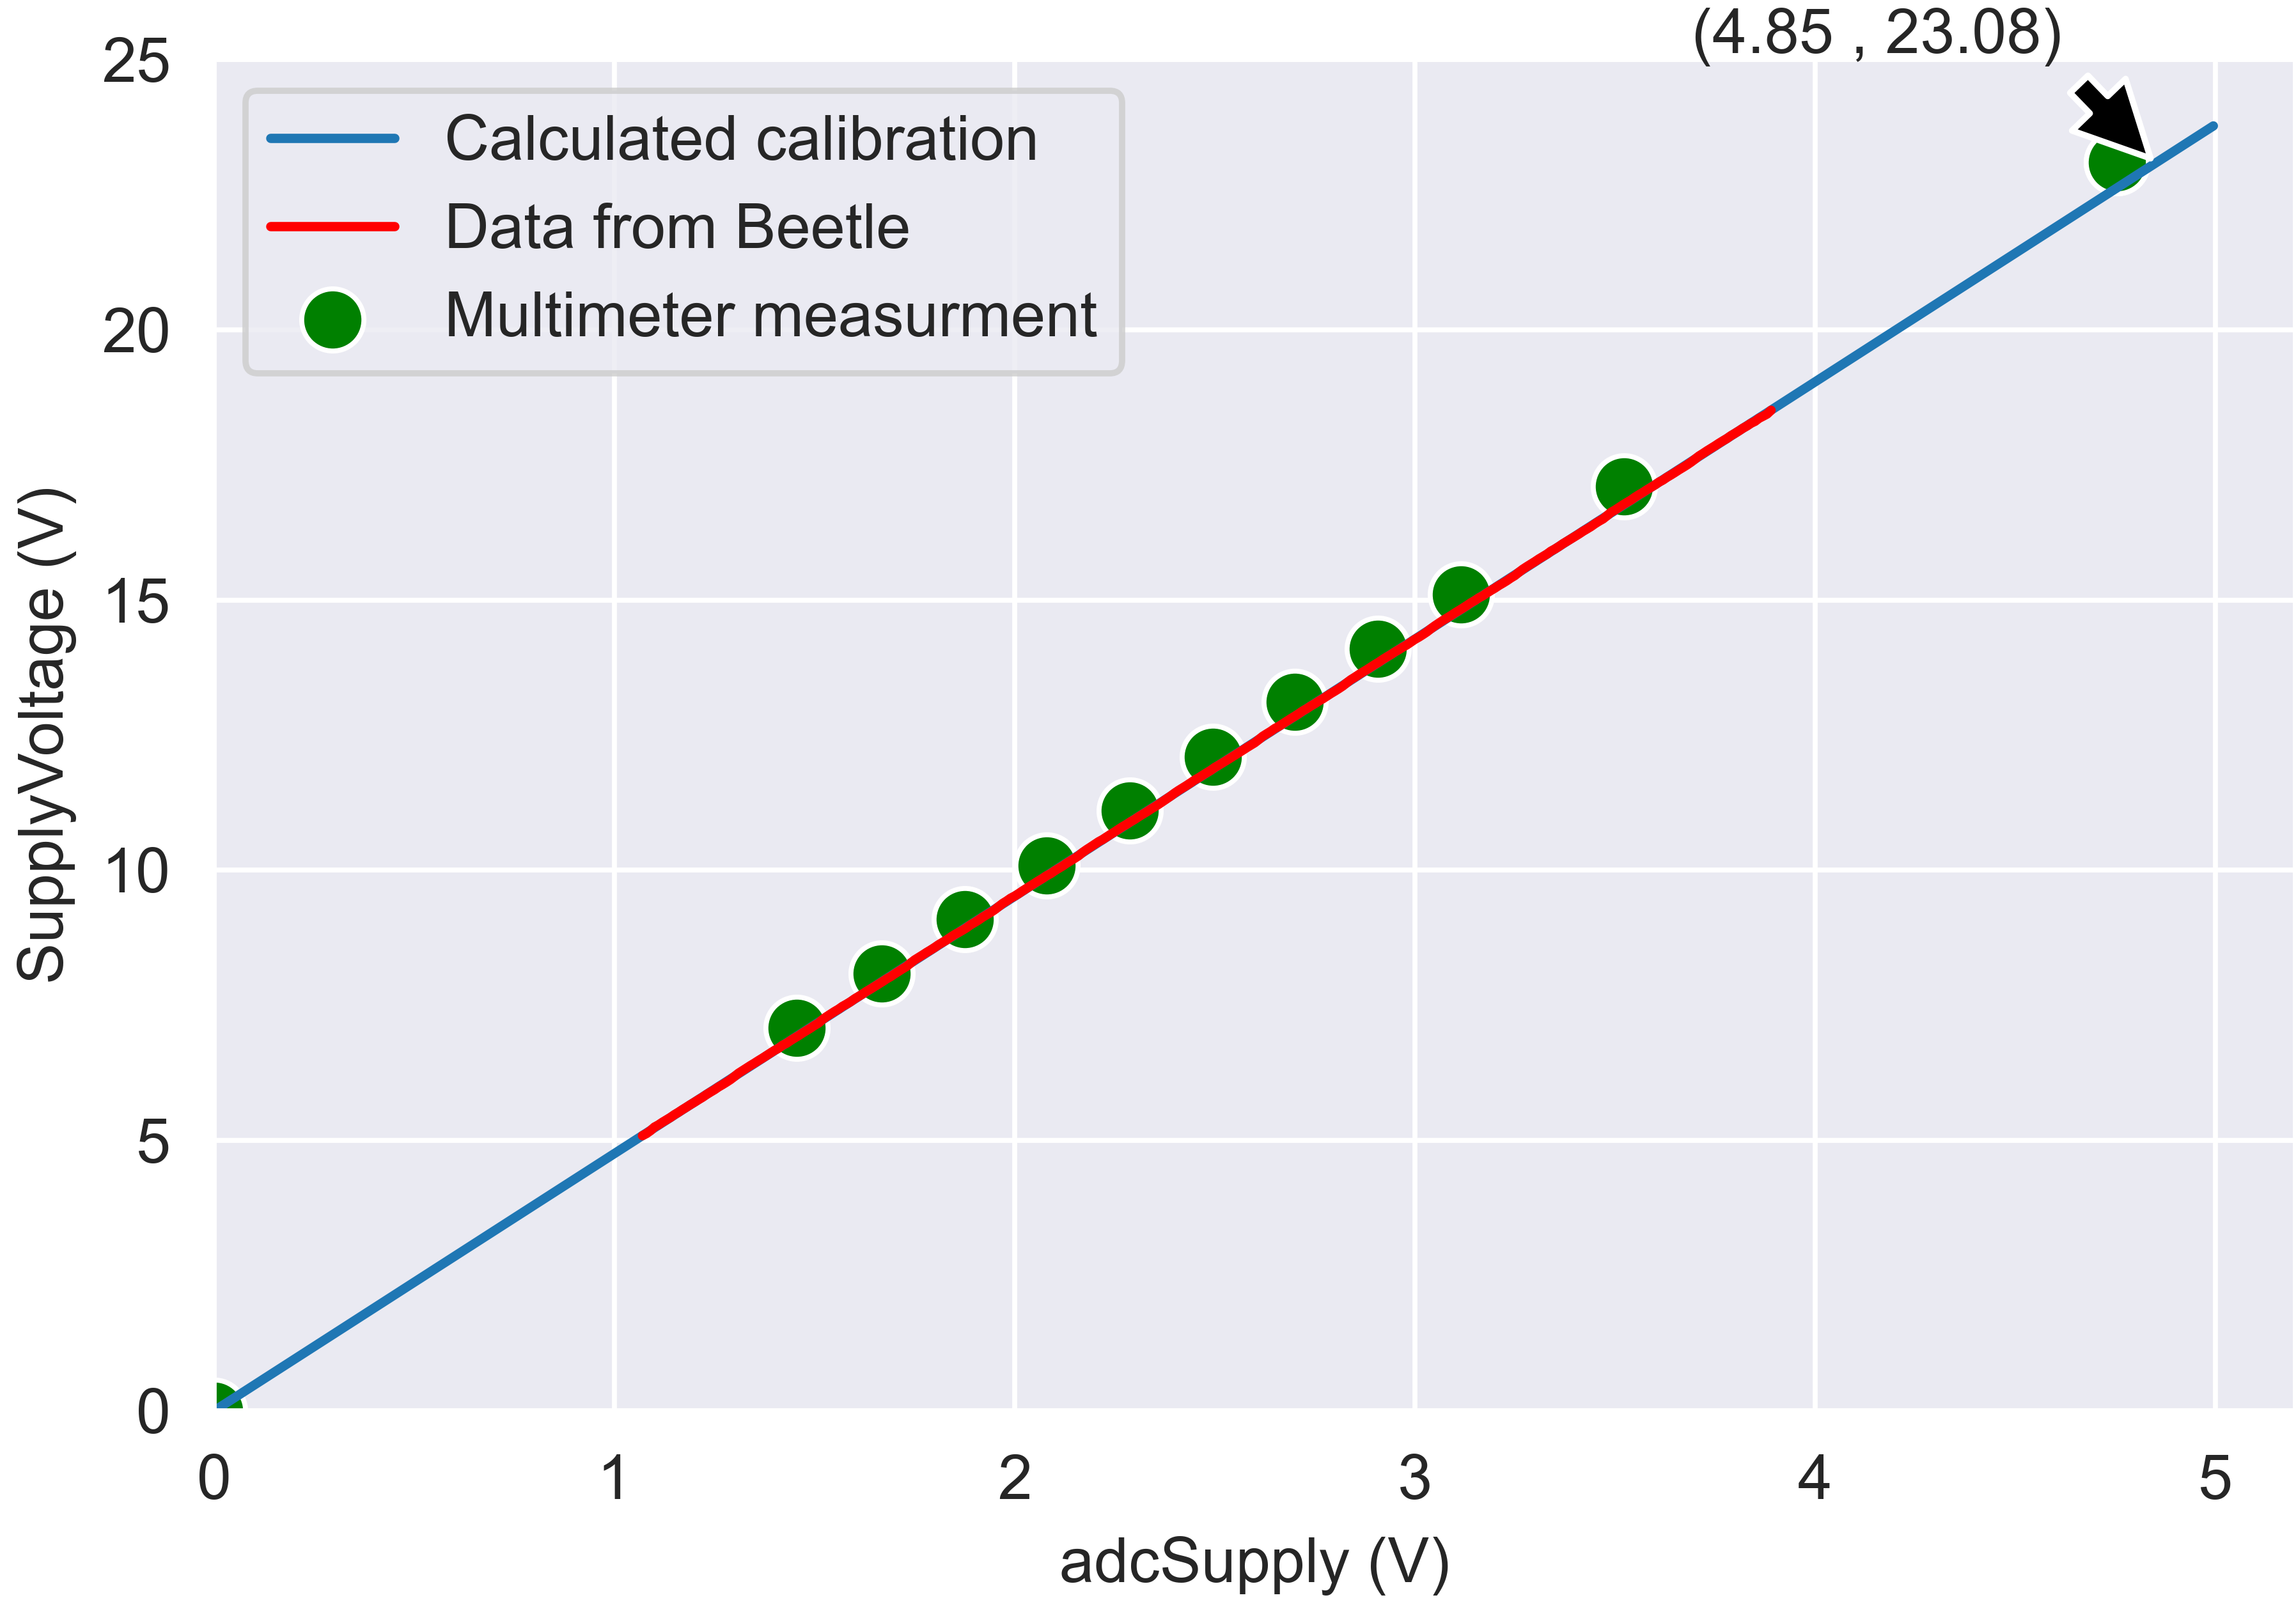
\includegraphics[width=0.38\textwidth]{./Figures/A8/supplyA8.png}
	\end{center}
	\caption{Supply ADC calibration}
	\label{fig:A8sup}
\end{wrapfigure}

The \textbf{supply voltage} starts at zero and reaches a maximum, a single measurement close to the maximum can be taken to determine the ratio of the adc input voltage to the actual supply voltage as can be seen in the following equation.
$V_{Supply} = V_{adcSupply} \times \frac{V_{measuredSup}}{V_{measuredADCSup}}$. Once again in figure \ref{fig:A8sup} it can be seen that the multimeter measurements very closely resembles the calibrated ADC values.
To calibrate the \textbf{current} to the correct value the value of $R_{shunt}$ was first determined from calculations. This was done by rearranging equation \ref{eq:refeq} to $R_{shunt}= \frac{(adcCurr-Vref)}{(50*currMeas)}$ where $V_{ref}$ is 1.753V and adcCurr and currMeas is 1.322V and -85mA. 

\begin{wrapfigure}{l}{0.38\textwidth}
	\begin{center}
		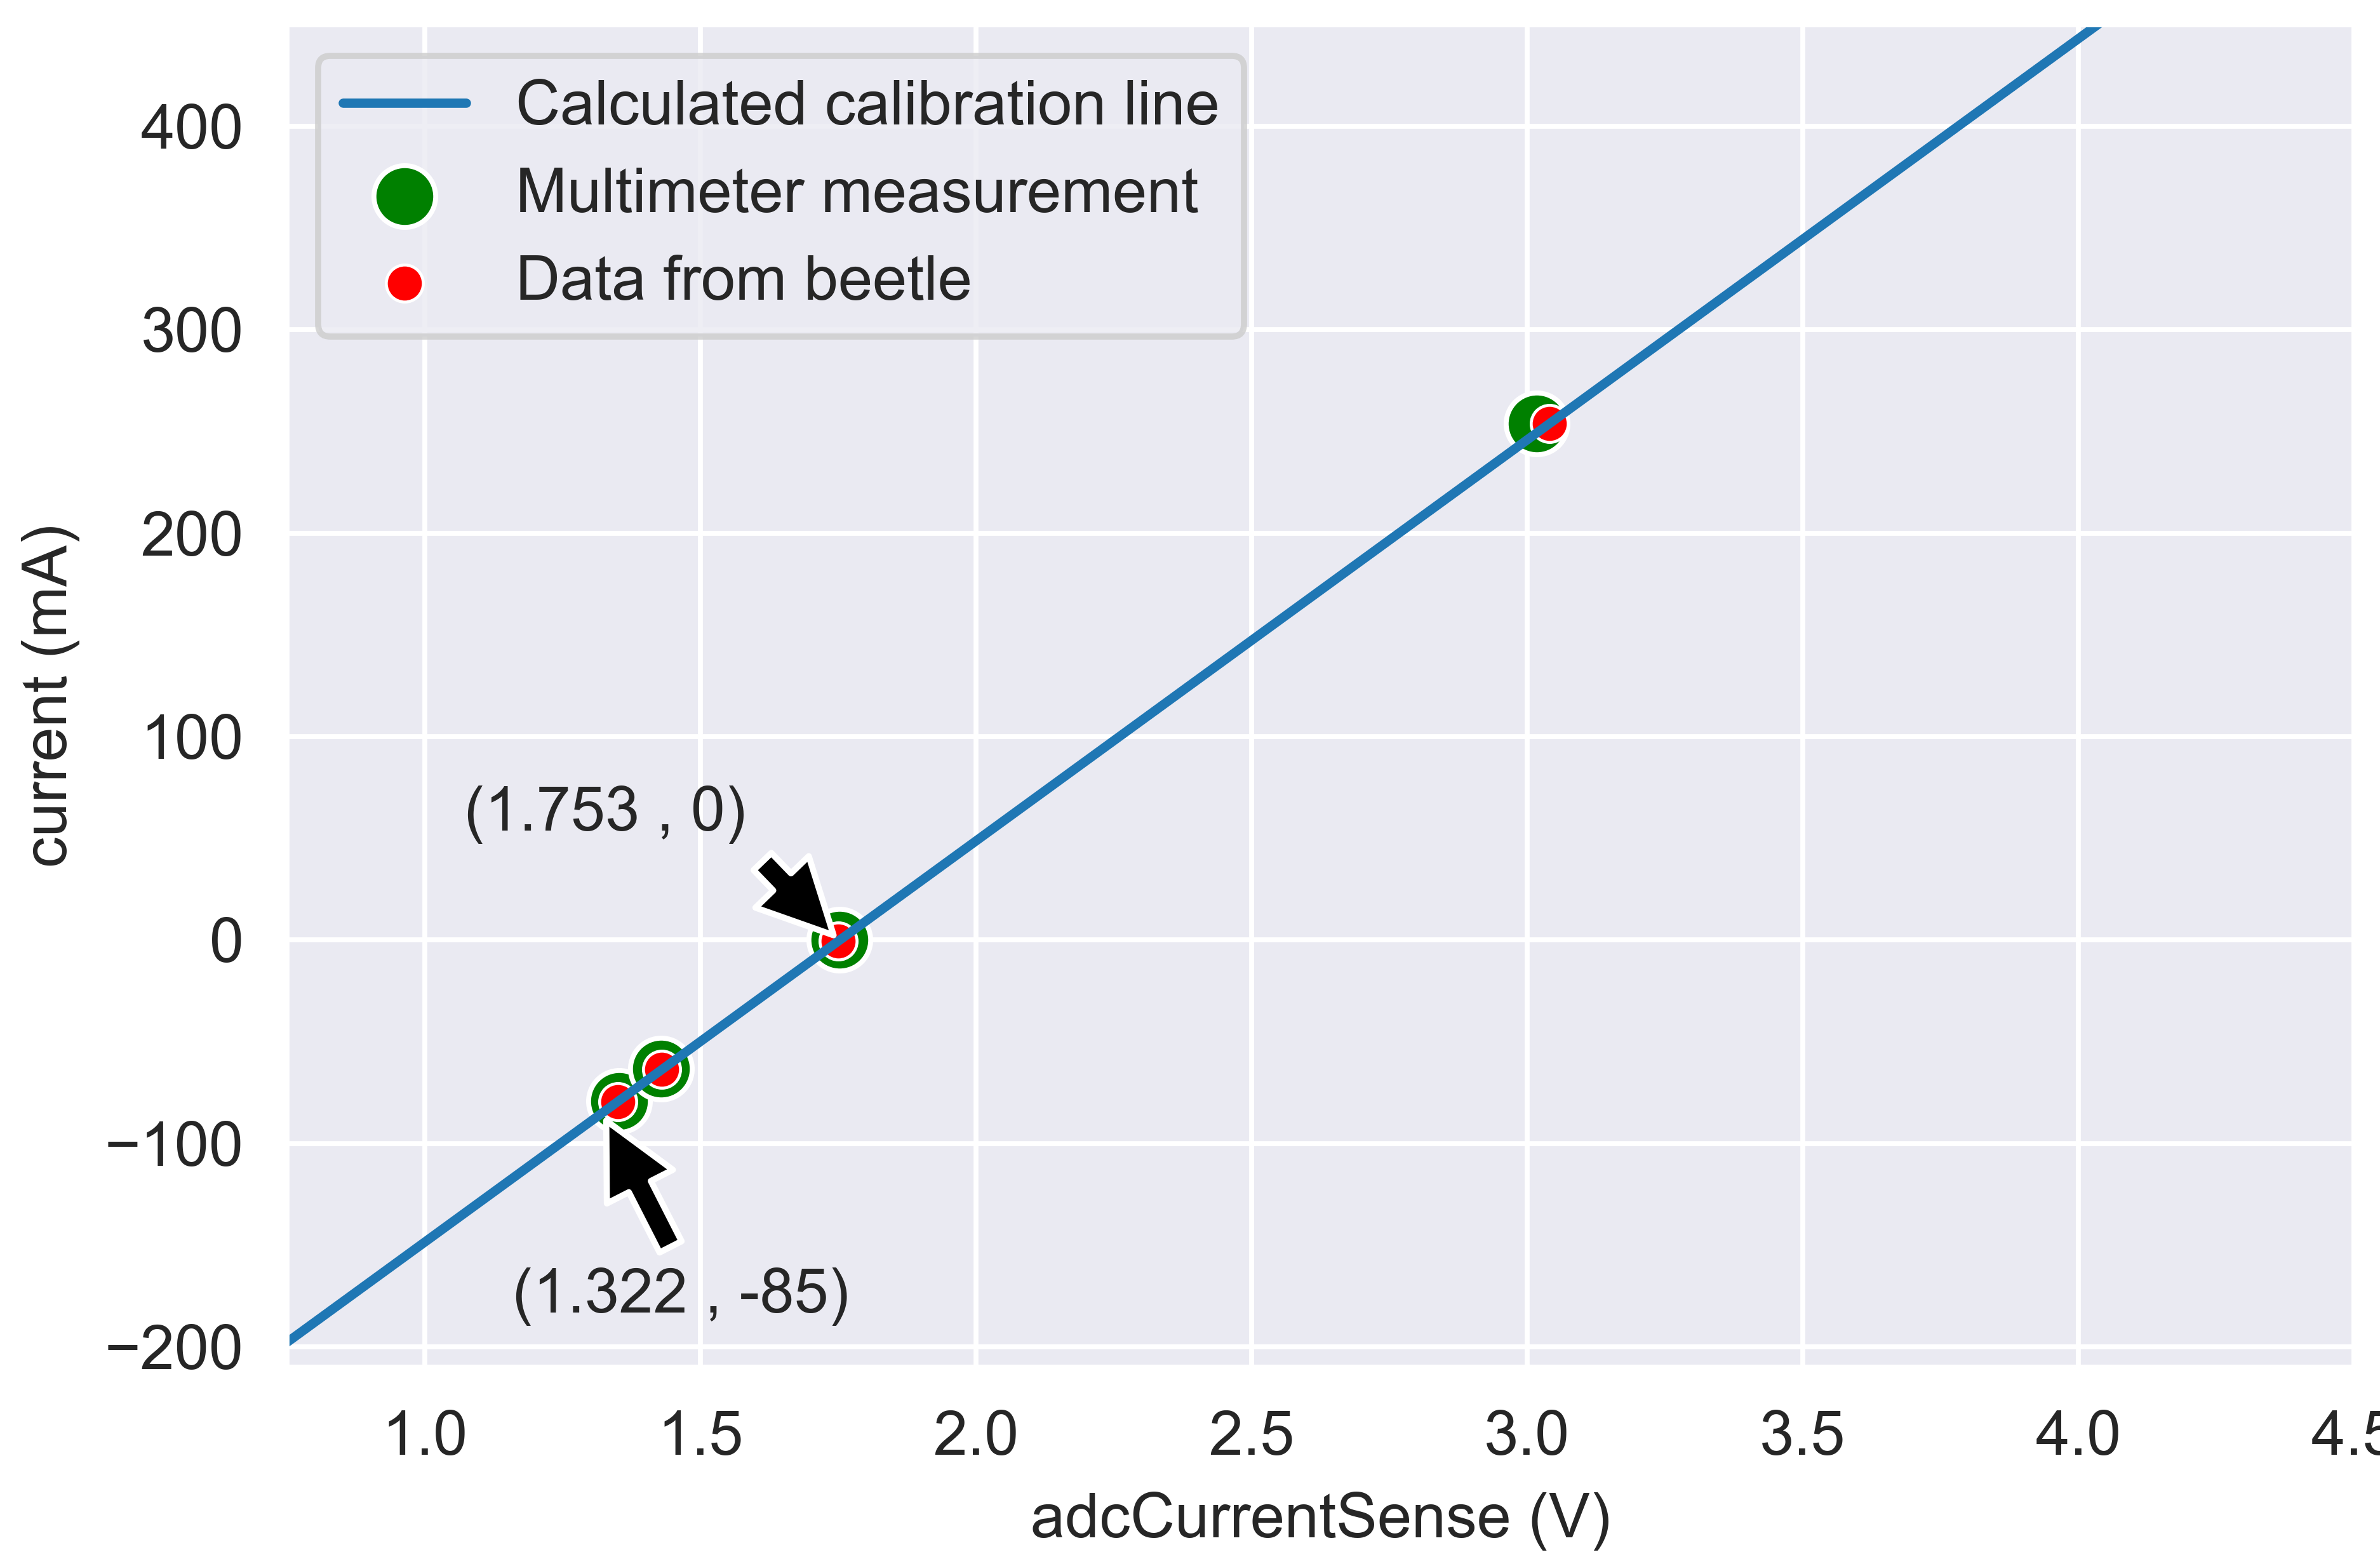
\includegraphics[width=0.38\textwidth]{./Figures/A8/currentA8.png}
	\end{center}
	\caption{Current ADC calibration}
	\label{fig:A8curr}
\end{wrapfigure}
The final equation used was  $Current = \frac{adcCurr-V_{ref}}{50*Rshunt}\times 1000$. From figure \ref{fig:A8curr} it can be confirmed that the calibrated values are very close to the multimeter measurements. 

The \textbf{LDR} value read does not need to be a specific output only 100 at its maximum brightness and 0 at its darkest. To achieve this the ADC value was divided by 10 and subtracted from 100. $light_{out}=100-ADC_{light}/10$. When the LDR is at its darkest (ADC measured just below 1000) it will be close to 0, and when it is at its brightest a value close to 100 will be achieved.
